\providecommand{\main}{../../../..}
\documentclass[\main/dresen_thesis.tex]{subfiles}

\begin{document}
  Multiple times in this thesis, two-dimensional experimental data sets with finite binning are presented.
  Often it is necessary for the proper evaluation to perform a coordinate transform on this data.
  When performing such transformations, it is for the data evaluation desired to have once again a rectangular grid.
  Care has to be taken how a rectangular bin in the original coordinate system is then represented in the new coordinate system.
  In the following, a pixel-splitting algorithm that was implemented for this purpose is presented.
  The algorithm performs the task for a given set of data, defined with respect to two coordinates, of applying an arbitrary (non-linear) coordinate transformation and saving the new data on an evenly spaced rectangular grid by splitting and distributing a given data point on different bins according to their area overlap.
  Furthermore, it propagates the monitor values in parallel, such that the rescaling can be performed after the rebinning and error estimates by Poissonian counting statistics can be further performed in the new coordinate system.

  The algorithm was conceived with the intention to transform data acquired at SuperADAM (\refsec{ch:lss:superadam})  and MARIA (\refsec{ch:lss:maria}) from the experimental space of the detector pixel coordinate $x$ and the incident angle $\alpha_i$ to either the reciprocal space ($q_x$, $q_z$) or the related coordinate space defined by incident and outgoing angle ($\alpha_i - \alpha_o$, $\alpha_i + \alpha_o$).
  In this case, the $x$ coordinate is defined on an evenly spaced grid, namely the pixel spacing of the detector, and $\alpha_i$ may be unevenly spaced, as it is up to the experiment at which specific angles a measurement is performed.
  To properly determine the specular scattering and subtract the diffuse scattering, it is desired that after coordinate transformation the data is given on an evenly spaced rectangular grid.

  \begin{figure}[tb]
    \centering
    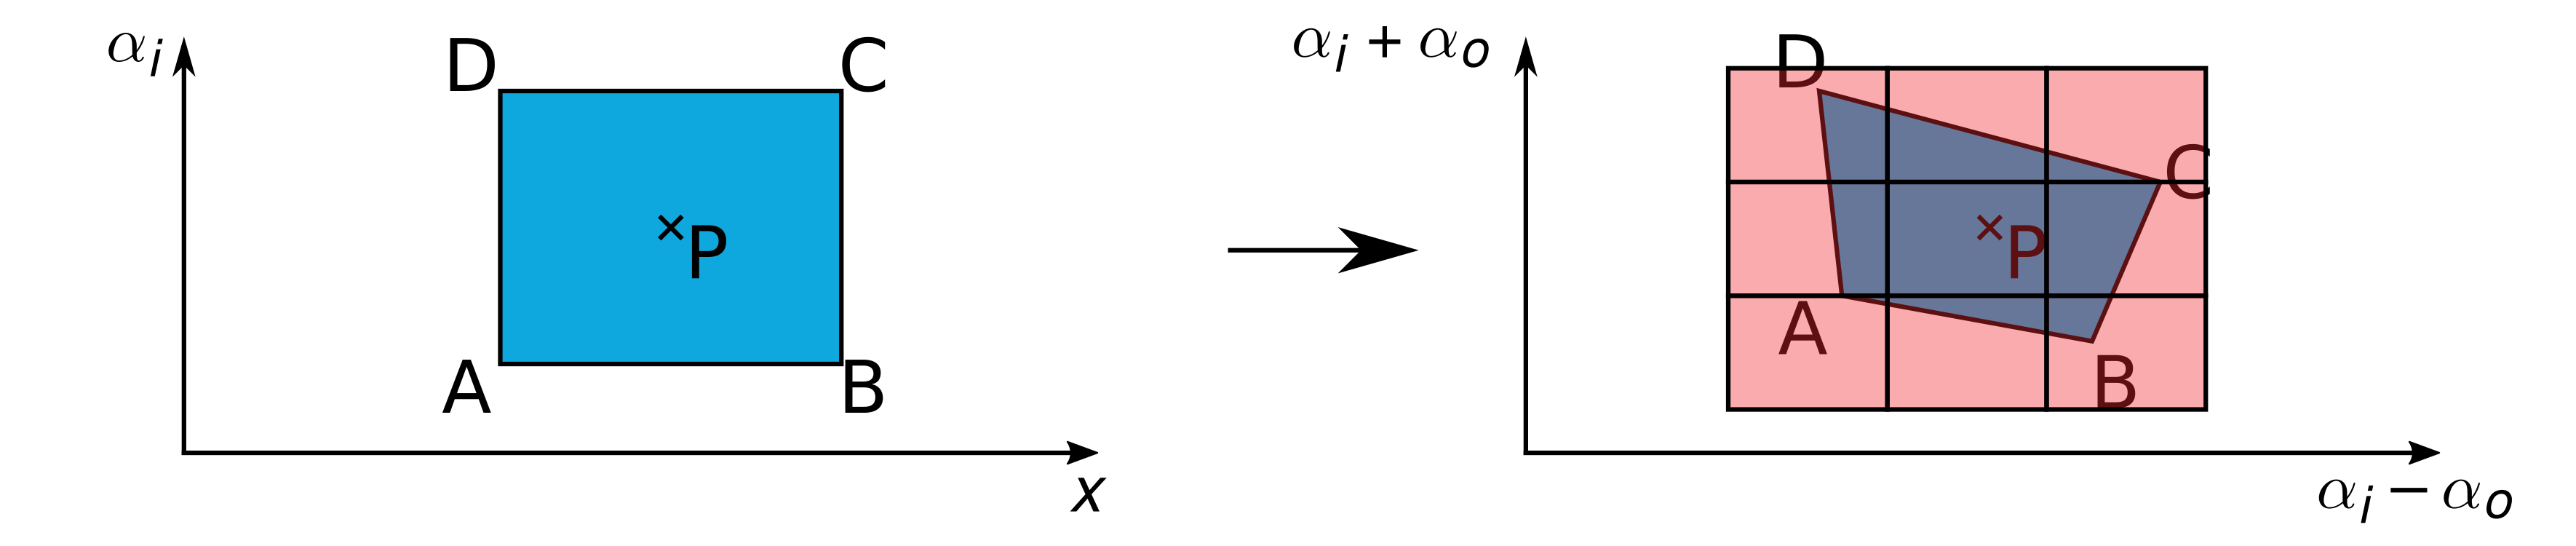
\includegraphics{rebinning_pixel}
    \caption{\label{fig:numericalMethods:rebinningPixelSplitting:pixelTransform}By a coordinate transformation the blue rectangular pixel, corresponding to data point P and bound by the rectangle ABCD, is mapped on the distorted pixel in the new coordinate space. In the pixel-splitting algorithm, the overlap areas of the distorted pixel with the new rectangular are determined and used to split the content of P onto the new pixels.}
  \end{figure}

  To describe the algorithm, we define for every measured data point on the original two-dimensional grid a pixel.
  The original pixel size is naturally given for the $x$ coordinate by the detector width and for $\alpha_i$ by the incident beam divergence.
  Within the pixel, the respective count of the data point and its monitor value are stored separately.
  For the new coordinate space an evenly spaced grid is prepared within the range of interest, and with the resolution one desires to have (being limited by the resolution of the original data).
  The algorithm then proceeds to loop over all pixels, and to apply the coordinate transformation for every corner point of the pixel.
  Within the new coordinate space the pixel is now no longer necessarily rectangular as sketched in \reffig{fig:numericalMethods:rebinningPixelSplitting:pixelTransform}.
  To divide the information contained in the distorted pixel onto the new rectangular grid, the area of the quadrilateral and the overlapping areas of the quadrilateral with respect to the new rectangular grid pixels are determined.

  \begin{figure}[tb]
    \centering
    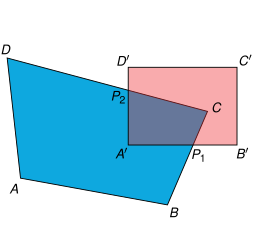
\includegraphics{rebinning_OverlapAreas}
    \caption{\label{fig:numericalMethods:rebinningPixelSplitting:overlapAreas}To determine the overlap of a general quadrilateral ($ABCD$) with a rectangular pixel ($A^\prime B^\prime C^\prime D^\prime $), the crossing points $P_1$ and $P_2$ are determined, thus giving the overlap from the polygon area of ($A^\prime P_1CP_2$).}
  \end{figure}

  Looking at the general case of an arbitrary quadrilateral and a rectangular bin as shown in \reffig{fig:numericalMethods:rebinningPixelSplitting:pixelTransform}, the overlap area is defined by determining the crossing points of both bins and by determining the corner points for both bins which are within the other bin.
  Together these points define a polygon, whose area represents the overlap area.
  To determine whether a corner point of the quadrilateral is within a rectangular bin is trivial.
  The more difficult question, if the corner point of an rectangular bin is inside an arbitrary polygon, is a known and efficiently solved problem in computer science known as the ray-casting algorithm \cite{Shimrat_1962_Algor}.
  The crossing of the edges are obtained geometrically by calculating for each edge of the quadrilateral the crossing with each of the the rectangular edges considering each as infinite straight lines, and checking afterwards whether the crossing points are within the bounds of the rectangular bin.
  Once the polygon points of the overlap boundary are obtained, the area is simply calculated by sorting the polygon points in a counter clockwise order and summing the cross-product of all neighboring points.

  Knowing the respective overlapping areas  of the distorted pixel of area  with the new grid, the count data contained in one pixel is divided proportionately onto the respective rectangular pixels.
  Thus, each rectangular grid $i$ then contains the count $C^\prime_i$, which is
  \begin{align}
    C^\prime_i \eq \sum_{j} C_j \frac{A_i^j}{A_j},
  \end{align}
  where $j$ is the index of the distorted pixel, $C_j$ it's respective count, $A_j$ it's respective area, and $A_i^j$ the overlap area of the rectangular and the distorted pixel.

  The monitor values $M^\prime_i$, are determined for the rectangular pixels of the new grid by taking the weighted mean of the contributing pixels
  \begin{align}
    M^\prime_i \eq \frac{\sum_{j} M_j \frac{A_i^j}{A_j}}{\sum_{j} \frac{A_i^j}{A_j}},
  \end{align}

  The algorithm conserves the total count number of the two-dimensional data, keeps the order of magnitude of the monitor value and doing this procedure, the count error in the respective pixels can be estimated by taking the square root of the new count values.
  For usability, the rebinning algorithm is implemented in Fortran90 and compiled for Python using the F2PY interface from NumPy \cite{Oliphant_2006_Guide}.
  The run time of the algorithm on a modern notebook for a common data set with $> 100000$ data points per image is less than $1 \unit{s}$ and therefore it's suitable for implementation in interactive coordinate transformation user interfaces.
\end{document}